\scanpage{100}

En effet, \deleted{on a}\inserted{sachant qu'on a} $y=\lambda x$, \unsure{i.e.} $x+iy=(a+\underline i b)x_0$, \deleted{\unsure{et}} avec $x_0=x$ \inserted{et $a+\underline i b=1+\underline i\lambda$} et on a $a^2+b^2\deleted{\unsure{\ne0}}=1+\lambda^2\ne0$ puisque, on doit avoir $\lambda^2\ne-1$, d'où nécessité. Pour Suffisance, si $x+iy=x_0(a+ib)$, i.e. $x=\deleted{\unsure{q}}ax_0,\ y=by_0$, on aura bien sûr $q(x)=q(y)={\unsure{a}}^{2}q(x_0)=0$

\figure{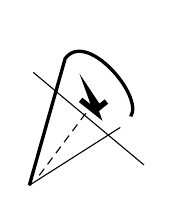
\begin{tikzpicture}[scale=.7]\draw[very thick] (0,0)--(.65,2.3) .. controls (1.04,2.83) and (2.08,1.62) .. (1.84,1.25);\draw (0,0)--(1.65,1.05) (.07,2.05)--(2.08,.37);\draw[densely dashed] (.18,.18)--(1.16,1.49);\draw[line width=2pt] (.93,1.55)--(1.22,1.32)--(1.10,1.65)--(1.26,1.41)--(1.40,1.52);\end{tikzpicture}}

O.K. \ldots

\deleted{\uline{Cas de la car 2} $S[\underline i]$ est alors can. isom. au schém. des \unsure{nbs} duaux, \inserted{$\underline i=1+\varepsilon$ donc} $\deleted{\unsure{\tilde X|X}}X^{S[\underline i]}$ est le fibré tangent à $X$.}

\deleted{On trouve}

\[
\begin{aligned}&\deleted{x+\underline i y=(\underbrace{x+y}_{z})+\varepsilon y\longmapsto[x,y]/q(x)}\\ &\deleted{(x+y\ne0\text{ i.e. }x\ne y)}\qquad\deleted{=[x+y,y]/q(y)}\\ &\deleted{z+\varepsilon y\longmapsto[z,y]/q(y)}\end{aligned}
\]

\[
\deleted{\unsure{\text{à}}\left\{\begin{aligned}&z\ne0\\ &\underbrace{q(y+z)=q(y)\unsure{,}\ne0}_{q(z)\deleted{\unsure{+|=}}\varphi(y,z)}\end{aligned}\right.}
\]

\deleted{\unsure{alors}}

\diagram{\begin{tikzcd}[ampersand replacement=\&,column sep=small,row sep=small] \deleted{\left\{\begin{aligned}\det u&=1\\\operatorname{Tr}u&=0\end{aligned}\right.\;(\Rightarrow u^2+1=0)}\arrow[r,leftrightarrow,"{?}"] \& \deleted{\left\{\begin{aligned}&x+\underline iy\quad q(x)=q(y)\ne0,\ \varphi(x,y)=0\\&\deleted{\unsure{y}}=\lambda\end{aligned}\right.}\\ \deleted{u=\deleted{\unsure{+}}[v,w]/\det v}\arrow[u,Rightarrow,"{?}"'] \& \deleted{\text{où }\left\{\begin{aligned}&\det v=\det w\ne0,\quad\operatorname{Tr}v=\operatorname{Tr}w=0\\ &\operatorname{Tr}vw=0\\ &\deleted{\unsure{k}v,w\ \text{pas de la forme }\lambda v,\ v+\underline i w}.\\ &\deleted{\unsure{v\ne v}}\quad v\ne w\end{aligned}\right.}\end{tikzcd}}

\[
\det[v,w]
\]

% archive sheet number: 99
